% !TEX root = pfe-book2.tex
%!TEX TS-program = pdflatex
%!TEX encoding = UTF-8 Unicode


\cleardoublepage
%\mainmatter
\chapter{Laws of Thermodynamics}
\label{ch-08}
\section{Conservation of Energy at the Molecular Level}

The laws of thermodynamics belong to the basic laws of nature. There are not many such laws. You can count them on the fingers of one hand.

The chief aim of science, including physics, of course is the search for the rules, regularities, general laws and the basic laws that govern nature. This search begins with observations or experiments. That is why we say that all of our knowledge is of an empirical or experimen­tal nature. 

Investigations and observations are followed by a search for generalization. Persistent brain work, meditation, calculations and inspiration enable us to find laws of nature. Next comes the third stage: from the general laws, we derive, in a strictly logical manner, the ensuing effects and special laws that can be checked by experiments. This, by the way, is what the explanation of a phenomenon consists of. To explain means to corre­late the particular with the general law.

A cherished goal of science has been, of course, suc­cessful attempts to reduce laws to the minimum number of postulates. Physicists tirelessly search for such oppor­tunities; they seek to express the whole sum of knowledge about nature in several concise and elegant formulas. Albert Einstein tried for about thirty years to unify the laws of gravitational and electromagnetic fields. The future will show whether or not this proves possible.

What, the are these laws of thermodynamics? Too brief a definition must necessarily be somewhat inac­curate. Maybe we approach the essence of the matter clos­est of all if we contend that thermodynamics is a study of the rules according to which bodies exchange energy. The laws of thermodynamics enable us to find strictly logical relations by mathematical means between the thermal and mechanical properties of bodies, and to es­tablish a number of vital principles concerned with the change of state of bodies. Perhaps, the most precise def­inition of the branch of physics we are about to give our attention to is the trivial statement: thermodynamics is the totality of knowledge that follows from the first and second laws of thermodynamics.

The first law of thermodynamics was formulated in a concise and expressive form back in the time when phys­icists preferred not to mention molecules. Such a formu­lation (which does not require us to ``get inside'' a body) is said to be phenomenological, i.e. one simply referring to the phenomena. The first law of thermodynamics con­stitutes a certain refinement and expansion of the energy conservation law.

We have established that a body has kinetic and po­tential energies, and that in a closed system, the sum of these energies -- the total energy -- can neither be de­stroyed nor created. Energy is conserved.

Except with respect to the motion of celestial bodies, we can contend without exaggeration that there are no phenomena in which mechanical motion is not accompa­nied with heating or cooling surrounding bodies. When a body is stopped by friction, its kinetic energy would seem, on the face of it, to be lost. This first impression is mis­leading, however. Actually, it can be proved that con­servation is maintained with absolute precision: the mechanical energy of the body has been utilized to heat the surrounding medium. What does this mean at the molec­ular level? Simply that the kinetic energy of the body has been transformed into kinetic energy of molecules. 

This seems clear enough, but what happens when we crush ice in a mortar with a pestle? We keep pounding and the thermometer reading remains at zero all the time. It would seem that the mechanical energy we exert has vanished. If not, what has happened to it? Again, we find a clear answer: the ice has been converted into water. This means that the mechanical energy was expended in rupturing the bonds between the molecules, and their internal energy has been changed. Each time we observe that the mechanical energy of a body has disappeared, we readily discover that this only seems to be so, and that actually mechanical energy has been converted into the
internal energy of the bodies being observed.

In a closed system, certain bodies can lose and others can gain internal energy. But the sum of the internal ener­gies of all the bodies added to their mechanical energies remains constant for the given system.

Now let us turn our attention away from mechanical energy. We consider two instants in time. At the first instant, the bodies were at rest, then certain events oc­curred, and at the second instant the bodies are again at rest. We are certain that the internal energy of all the bodies in the system remained constant. But some bodies have lost and others have acquired energy. This could happen in two ways. Either one body performed mechanical work on another (for example, by compressing or stretching it), or one body transferred heat to another body.

The first law of thermodynamics states that the change in the internal energy of a body is equal to the sum of the work done on the body plus the heat transferred to it.

Heat and work are two different forms in which energy can be transferred from one body to another. Heat exchange is accomplished by disordered collisions of molecules. Mechanical energy is transmitted with the mole­cules of one body aligned in orderly ``rows and ranks'' transferring their energy to another body.

\section{How Heat Is Converted into Work}

The word ``heat''”in this heading has been employed somewhat carelessly. As mentioned immediately above, heat is a form of energy transfer. Consequently, a more proper formulation of the question would be: How to convert thermal energy, i.e. kinetic energy of molecular motion, into work. But the word ``heat'' is customary, concise and expressive. We hope the reader will not be confused if we continue to apply the word in the sense we have just accurately defined.

There is certainly plenty of heat around us. But, unfortunately, all of this energy of molecular motion is ab­solutely useless insofar as it cannot be converted into work. Such energy cannot be ranked in any way among our energy resources. Let us look into this matter.

A pendulum which has been deflected from its equilib­rium position will sooner or later come to rest, a wheel of an upside-down bicycle, which has been spun by hand, will make a lot of turns, but it, too, will eventually stop moving. There is no exception to the following important law: all the spontaneously moving bodies surrounding us will eventually come to rest.\footnote{Here, of course, we do not have in mind a uniform translatory motion or a uniform rotation of a system of bodies as a whole.}

If there are two bodies, one heated and the other cold, heat will be transferred from the former to the latter until their temperatures are equalized. Then the heat trans­fer will cease and the states of the bodies will stop changing. Thermal equilibrium will set in.

There is no phenomenon whereby a body spontaneous­ly leaves a state of equilibrium. A wheel on an axle at rest never starts turning by itself. Neither does it happen that an ink-well on a table warms up by itself.

The tendency towards equilibrium implies that events take a natural course: heat passes from a hot body to a cold one, but cannot spontaneously pass from a cold bo­dy to a hot one.

As a result of air resistance and friction at the suspen­sion, the mechanical energy of an oscillating pendulum will be converted into heat. However, not under any con­ditions will a pendulum begin swinging at the expense of the heat of the surrounding medium. Bodies come to a state of equilibrium, but cannot leave it spontaneously.

This law of nature shows at once what part of the energy surrounding us is absolutely useless. This is the energy of the thermal motion of the molecules of those bodies which are in a state of equilibrium. Such bodies are incapable of converting their energy into mechanical motion.

This part of the energy is immense. Let us calculate the value of this ``inaccessible'' energy. If the tempera­ture is lowered by one degree, then a kilogram of earth, having a heat capacity of \SI{0.2}{\kilo\calorie\per\kilo\gram}, loses \SI{0.2}{\kilo\calorie}. A relatively small figure. However, let us estimate how much energy we would obtain if we were able to cool by only one degree a substance with the mass of the Earth, i.e. \SI{6d24}{\kilo\gram}. Multiplying we obtain an im­mense figure: \SI{1.2d24}{\kilo\calorie}. In order that you might picture this value, let us state at once that at the present time, the yearly energy output of all the electric power stations in the world is equal to \numrange{d15}{d16} \si{\kilo\calorie}, i.e. about a thousand million times less.

We needn’t be astonished by the fact that such calcu­lations act hypnotically on poorly informed inventors. We have spoken above of attempts to construct a perpet­ual motion machine (``perpetuum mobile'') creating work out of nothing. Operating with the principal proposi­tions of physics following from the law of conservation of energy, one cannot possibly refute this law with the creation of a perpetual motion machine (we shall now call it a \emph{perpetual motion machine of the first kind}).

The same sort of error is also committed by certain cleverer inventors, who create models of machines performing mechanical motion at the expense of nothing but by cooling the medium. Such, alas, unrealizable machines are called \emph{perpetual motion machines of the second kind}. 

Here, too, a logical error is committed, since the inventor bases himself on laws of physics, which are consequences of the law by which all bodies tend towards a state of equilibrium, and with the aid of these laws, tries to refute the foundations on which they are based.

Thus, it is impossible to produce work by merely taking heat from a medium. In other words, a system of bodies in equilibrium with each other is energetically barren.

Hence, in order to obtain work, it is first of all neces­sary to find bodies which are not in equilibrium with their neighbours. Only then will one succeed in realizing a process of transferring heat from one body to another or converting heat into mechanical energy.

The creation of an energy flux is a necessary condition for obtaining work. In the ``path'' of such a flux a conver­sion of some of the energy of bodies into work is possible. Therefore, the energy of only those bodies which are not in equilibrium with the surrounding medium is ranked among the energy reserves which are of use to people.

The law which we have just expounded, the impossi­bility of building a perpetual motion machine of the sec­ond kind, is called the second law of thermodynamics. So far we have expressed it in the form of a phenomenological rule. But since we know that bodies consist of mole­cules and that the internal energy is the sum of the kinet­ic and potential energies of the molecules, the sudden appearance of some kind of ``additional'' law may seem strange. Why is the law of conservation of energy formu­lated for molecules insufficient to explain all phenomena in nature?

In short, this poses the following question: Why do molecules behave so that when left to themselves they tend towards a state of equilibrium?

\section{Entropy}
This question is very important and interesting. In order to answer it, we will have to begin from afar. Frequently encountered events that occur at every turn are said to be highly probable. On the contrary, events
that occur thanks to a rare coincidence are regarded as improbable.
An improbable event does not require a display of any supernatural forces whatsoever. There is nothing impos­sible about it, nothing contradicting the laws of nature. And nevertheless, in many cases we are perfectly sure that the improbable is identical with the impossible.

Consider a lottery prize-list. Count the number of win­ning tickets whose numbers end with a 4, 5 or 6. You will not be the least bit surprised when you find that approxi­mately one-tenth of the winning tickets correspond to each digit. Well, but perhaps tickets with numbers ending with a 5 were to make up one-fifth of the winners, instead of one-tenth? Unlikely, you say. Well, and if half of the winning tickets were to have such numbers? No, that would be absolutely improbable and therefore, also impossible.

Reflecting on what conditions are necessary for an event to be probable, we arrive at the following conclusion: the probability of an event depends on the number of ways in which it can be realized. The greater this num­ber, the more frequently will such an event occur.

More precisely, the \emph{probability} is the ratio of the num­ber of ways of realizing a given event to the number of ways of realizing all possible events.

Write down the numbers from 0 to 9 on ten cardboard discs and place them in a sack. Now pull out a disc, note its number and put it back in the sack. This is very much like a lottery drawing. It can be confidently said that you will not draw one and the same number, say, seven times in a row, even if you devote an entire evening to this boring occupation. Why? The drawing of seven identical numbers is an event which is realizable in only ten ways (7 zeros, 7 ones, 7 twos, etc.). But there are a total of \num{d7} possible ways of drawing seven discs. Therefore, the probability of drawing seven discs in a row with identical numbers is equal to $10/\num{d7} = \num{d-6}$, i.e. only one-millionth.

If black and white grains are poured into a box and mixed with a shovel, the grains will very soon be distri­buted uniformly throughout the entire box. Scooping up a handful of grains at random, we shall find approxi­mately the same number of white and black grains in it. No matter how much we mix them, the result will always be the same -- uniformity is preserved. But why doesn’t the separation of the grains take place? Why won’t we succeed in driving the black grains to the top and the white grains to the bottom by means of a prolonged mix­ing? Here, too, it is entirely a matter of probability. The state in which the grains are distributed disorderly, i.e. black and white grains are uniformly intermingled, can be realized in an enormous number of ways and, consequently, possesses the greatest probability. On the contrary, the state in which all the white grains are on the top and all the black grains at the bottom is unique. Therefore, the probability of its realization is negligibly small.

We can easily pass from grains in a sack to the mole­cules that bodies are made of. The behaviour of mole­cules is subject to chance. This can be seen particularly clearly in the case of gases. As we know, gas molecules collide randomly and move in all possible directions, first with one speed and then with another. This eternal thermal motion continually reshuffles the molecules, mixes them like a shovel mixes the grains in a box.

The room in which you are now is filled with air. Why can’t it happen at some moment that the molecules in the lower half of the room pass into the upper half—under the ceiling? Such a process is not impossible -- it is very im­probable. But what does very improbable mean? If such a phenomenon were even a thousand million times less probable than a disordered distribution of molecules, someone might nevertheless observe it. Will we really observe such a phenomenon?


A computation shows that such an event for a \SI{1}{\centi\meter\cubed} vessel in volume takes place once in $10^{3 \times 10^{19}}$ cases. It hardly pays to make a distinction between the words “extremely improbable” and ``impossible''. For the num­ber written above is unimaginably great; if we divide it by the number of atoms not only on the Earth but also in the entire solar system, it will still remain enor­mous.

But what will the state of the gas molecules be? The most probable one. And the most probable state will be that which is realizable in the greatest number of ways (the molecules will all be distributed at random) for which there are approximately the same numbers of mol­ecules moving to the right as to the left, upwards as downwards, for which one finds identical numbers of molecules in equal volumes, the same proportion of fast and slow molecules in the upper and lower halves of the vessel. Any deviation from such a disorder, i.e. from the random intermingling of molecules with respect to position and velocity, is linked with a decrease in probability, or, more concisely, is an improbable event.

On the contrary, phenomena linked with an intermin­gling, with the creation of disorder out of order increase the probability of state. Hence, it is these phenomena that will determine the natural course of events. The law of the impossibility of a perpetual motion machine of the second kind and the law by which all bodies tend towards an equilibrium state receive their explanation. Why is mechanical motion transformed into thermal? Simply because mechanical motion is ordered and thermal is disordered. The transition from order to disorder in­ creases the probability of state.

Physicists called the quantity characterizing the degree of order and related by a simple formula to the number of ways of creating states \emph{entropy}. We shall not give the for­mula, but shall only say that the greater the probability, the greater the entropy.

The law of nature which we are now discussing asserts: all natural processes proceed in such a way that the probability of state increases. In other words, this same law of nature can be formulated as the law of increasing entropy.

The law of increasing entropy is one of the most im­portant laws of nature. From it follows, in particular, the impossibility of constructing a perpetual motion machine of the second kind, or, which is the same, the assertion that bodies left to themselves tend to a state of equilibrium. The law of increasing entropy is the same second law of thermodynamics. Only its formulation is different, but its content is the same. What is more important is that we have given an interpretation of the second law of thermodynamics at the molecular level.

In a certain sense, the union of these two laws ``under a single banner'' was quite fortunate. For the law of con­servation of energy is an absolute law. But as for the law of increasing entropy, as follows from what has been said above, it is applicable only to sufficiently large collections of particles and is simply impossible to formulate for individual molecules.

The statistical (this means pertaining to a large col­lection of particles) character of the second law of ther­modynamics does not in the least diminish its signifi­cance. The law of increasing entropy predetermines the di­rection of processes. In this sense, entropy may be called the managing director of natural resources, while energy serves as its bookkeeper.

\section{Fluctuations}
We have seen that spontaneous processes bring a sys­tem to its most probable state, i.e. to the growth in en­tropy. After the entropy of a system has become maximum, equilibrium is reached.

But a state of equilibrium does not by any means im­ply internal rest. An intensive thermal motion takes place within the system. Therefore, strictly speaking, any physical body ``stops being itself'' at each instant: the mutual distribution of its molecules at every succes­sive moment is not the same as it was at the preceding one. Consequently, the values of all physical quantities are conserved only ``on the average''; they are not exactly equal to their most probable values, but vary around them. Deviations from the most probable values at equi­librium are called \emph{fluctuations}. The values of the various fluctuations are extremely negligible. The greater the value of a fluctuation, the less probable it is.


The average value of a relative fluctuation, i.e. the fraction of the magnitude of the physical quantity of interest by which it can change as a result of the chaotic thermal motion of molecules, can be approximately
represented by the expression $1/\sqrt{N}$ , where $N$ is the number of molecules in the body, or in that part of it, which we are investigating. Therefore, fluctuations are appre­ciable for systems consisting of a small number of mole­cules, and completely insignificant for large bodies containing millions of millions of millions of molecules.

The formula $1/\sqrt{N}$ shows that in one cubic centimetre of a gas, the density, pressure, temperature and also any other properties can change by $1/\sqrt{3 \times 10^{19}}$, i.e. by not more than \num{d-8}\%. Such fluctuations are too small to be detected experimentally. However, things are entirely different for a volume of a cubic micrometre. Here $N = \num{3d7}$ and fluctuations will attain measurable val­ues of the order of hundredths of a percent.

A fluctuation is an ``abnormal'' phenomenon in the sense that it implies a transition from a more probable state to a less probable one. In the course of a fluctuation, heat transfers from a cold body to a hot one, the uniform dis­tribution of molecules is violated and an ordered motion sets in.

Will someone perhaps succeed in constructing a perpet­ual motion machine of the second kind on the basis of these violations?

Let us imagine, for example, a tiny turbine placed in a rarefied gas. Can’t we arrange things in such a way that this small machine would react to all fluctuations in an arbitrary but fixed direction? For example, so that it would rotate if the number of molecules flying to the right became greater than the number of molecules moving to the left? Such small tremors might be accumulated, eventually giving rise to work. The law asserting the impossibility of a perpetual motion machine of the second kind would be refuted.

But, alas, such a mechanism is impossible in princi­ple. A detailed examination, taking into account the fact that the turbine would have its own fluctuations (the greater, the smaller its dimensions), shows that fluctua­tions can never perform any work whatsoever. Although violations of the tendency towards equilibrium continual­ly arise around us, they cannot change the inexorable course of physical processes in the direction increasing the probability of state, i.e. entropy.

\section{Who Discovered the Laws of Thermodynamics!}
Here it is impossible to limit ourselves to a single name. The second law of thermodynamics has its own history. Here, too, just as in the history of the first law of thermodynamics, the name of the Frenchman Sadi Carnot should be mentioned first of all. In 1824, he pub­lished a work entitled \emph{Reflections on the Motive Power of Fire} at his own expense. It was first demonstrated in this work that heat cannot pass from a cold body to a warm one without the consumption of work. Carnot also showed that the maximum efficiency of a heat engine is determined only by the difference in the temperatures of the heater and the cooling medium.

Only after Carnot’s death in 1832 did other physicists pay attention to this work. However, it had little influ­ence on the further development of science because all of Carnot’s writings were based on the recognition of an indestructible and uncreatable ``substance'' -- caloric.

Only after the work of Mayer, Joule and Helmholtz, who established the law of equivalence of heat and work, did the great German physicist Rudolf Clausius (1822-1888) arrive at the second law of thermodynamics and formulate it mathematically. Clausius introduced the concept of entropy and showed that the essence of the second law of thermodynamics can be reduced to the inevitable growth of entropy in all real processes.

The second law of thermodynamics permits one to for­mulate a number of general laws which all bodies should obey, regardless of their structures. However, there still remains the problem of finding the relationship between the structure of a body and its properties. The branch of physics, which is called \emph{statistical physics}, gives an answer to this question.

It is clear that in calculating physical quantities describing a system consisting of millions of millions of millions of particles, a new approach is absolutely nec­essary. In fact, it would be pointless, not to say complete­ly impossible, to follow the motions of all the particles and describe this motion with the aid of formulas of me­chanics. However, it is precisely this enormous number of particles which enables us to apply new ``statistical'' methods to the study of bodies. These methods widely use the concept of the probability of events. The founda­tions of statistical physics were laid down by the outstand­ing Austrian physicist Ludwig Boltzmann (1844-1906). In a series of papers, Boltzmann showed how the indicated program can be carried out for gases.

The statistical interpretation of the second law of ther­modynamics given by Boltzmann in 1877 was the logi­cal culmination of these investigations. The formula relating the entropy and probability of state of a system was carved out on Boltzmann’s tombstone.


%\newpage

\begin{center}
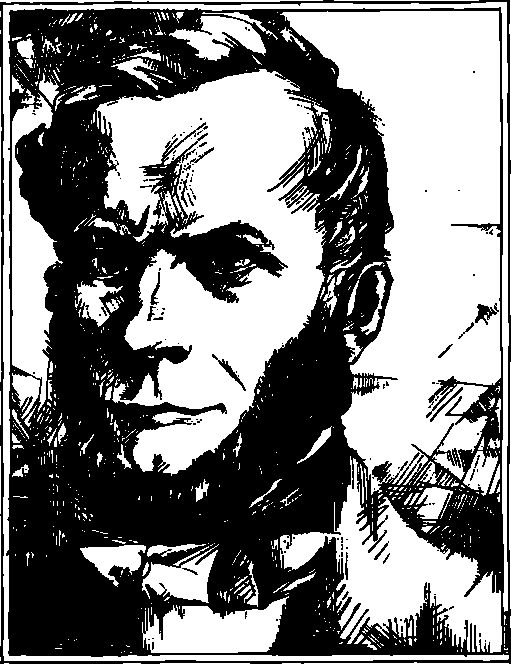
\includegraphics[width=0.8\textwidth,angle=-0.05]{figures/clausius.pdf}
\end{center}
{\small \textsf{{Rudolf Clausius [1822-1888]} -- \textsf{\footnotesize an outstanding German theoretical physicist. Clausius was the first to accurately formulate the second law of thermodynamics: in 1850, in the form of the thesis of the impossibility of heat being spontaneously transmitted from a colder body to a hotter one, and in 1865, with the aid of the concept of entropy which he introduced. Clausius was one of the first to consider the questions of the heat capacity of polyatomic gases and the thermal conductivity of gases. Clausius' work in the kinetic theory of gases contributed to the development of statistical concepts of physical processes. A series of interesting in­vestigations into electrical and magnetic phenomena are due to Clausius.}}}

It would be difficult to overestimate the scientific achievement of Boltzmann, who discovered completely new paths in theoretical physics. Boltzmann’s investigations were subjected to ridicule during his lifetime by conservative German professors: at that time, atomic and molecular conceptions were regarded by many as na\"ive. Boltzmann committed suicide, and the role played by the situation just described was undoubtedly far from the least important.

The edifice of statistical physics was perfected to a considerable degree by the work of the outstanding Amer­ican physicist Josiah Willard Gibbs (1839-1903). Gibbs generalized Boltzmann’s methods and showed how one might extend the statistical approach to all bodies.

Gibbs’ last paper appeared at the beginning of the 20th century. A very modest researcher, Gibbs published his papers in the proceedings of a small provincial uni­versity. A considerable number of years had passed until his remarkable investigations were made known to all physicists.

Statistical physics has shown the way in which one can calculate properties of bodies consisting of a given num­ber of particles. Of course, it should not be thought that these computational methods are all-powerful. If the nature of the motion of the atoms in a body is very complicated, as is the case for liquids, the actual computa­tion becomes unfeasible in practice.